\begin{mainquestion}{nmosbias}{NMOS Bias Circuit}

\questionpoints Consider the circuit below, where:
\[
k_n = 5\,\text{mA/V}^2, \qquad V_{tn} = 0.9\,V, \qquad V_{DD}=9V
\]

\begin{center}
    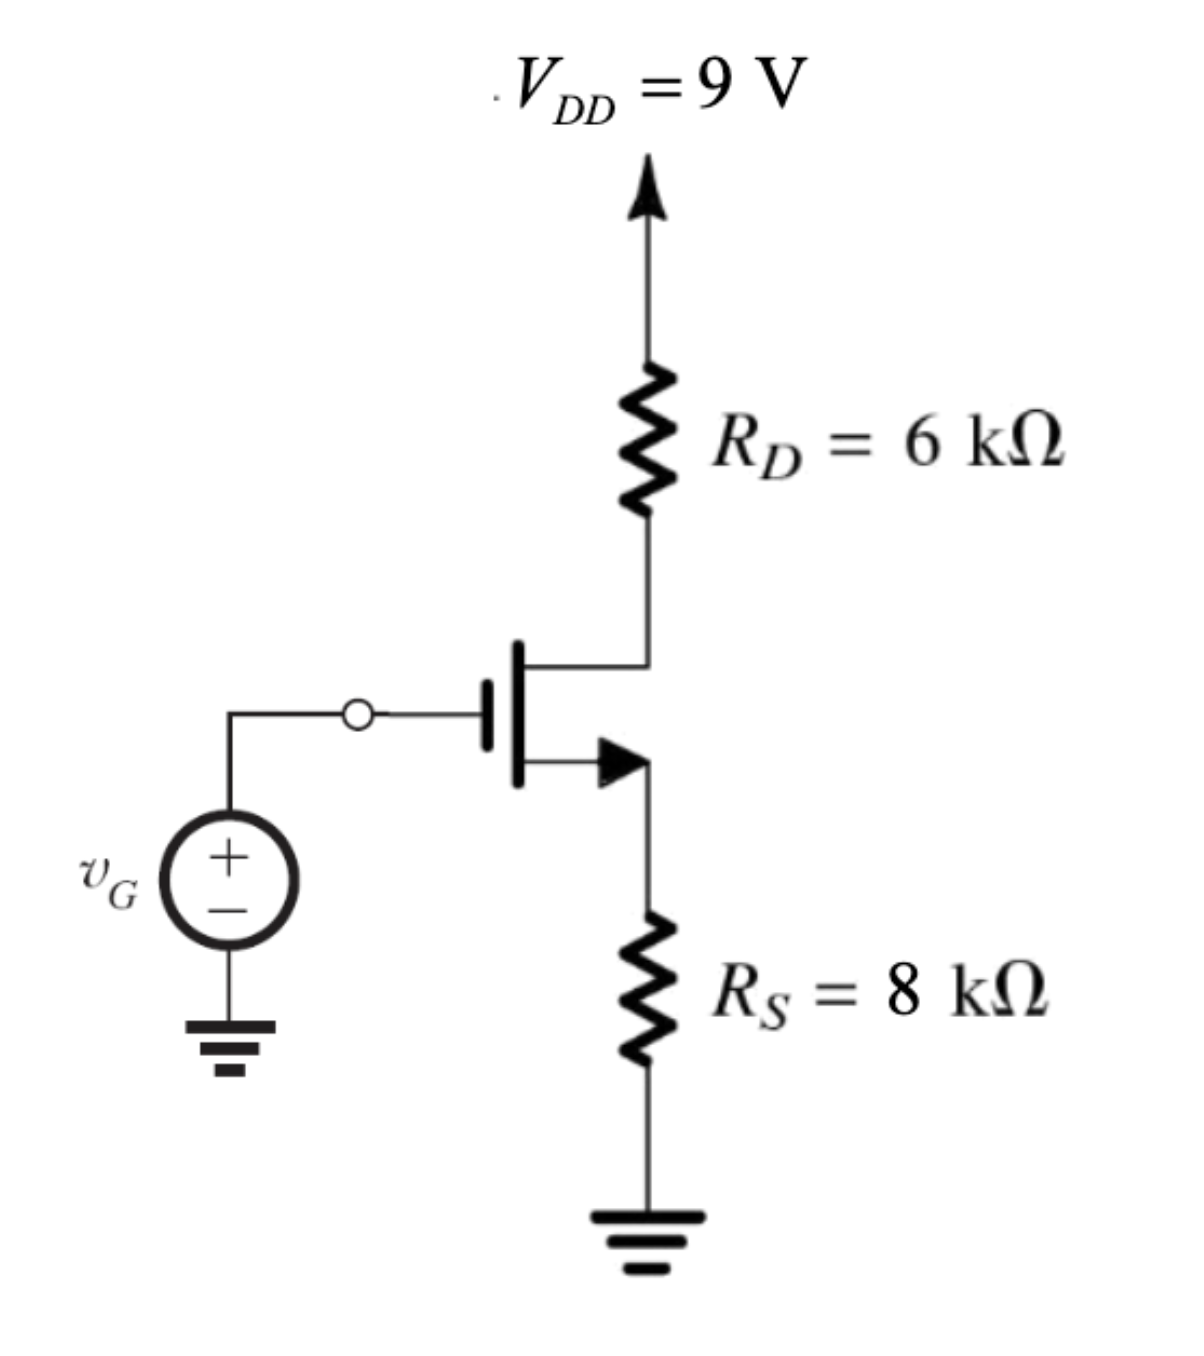
\includegraphics[width=0.6\textwidth]{q2.png}
\end{center}

%-----------------------------------------

% =========================================================
\begin{partquestion}{findvs}
{Find the drain and source voltages for the circuit if a biasing gate voltage $V_G=3V$ is used.}

\begin{answer}
Assume the transistor operates in saturation.  
The same current flows through $R_D$ and $R_S$:

\[
i_D = \frac{V_{DD}-V_D}{6k\Omega} = \frac{V_S}{8k\Omega}
\]

Thus:

\[
i_D = \frac{V_S}{8k\Omega}
\]

In saturation (valid only if $V_{GS}>V_t$):

\[
i_D = \frac{1}{2}k_n(V_{GS}-V_t)^2
\]

\[
V_{GS} = V_G - V_S = 3 - V_S
\]

\[
i_D = \frac{1}{2}(5)(3 - V_S - 0.9)^2
= \frac{5}{2}(2.1 - V_S)^2
\]

Set equal:

\[
\frac{V_S}{8k} = \frac{5}{2}(2.1 - V_S)^2
\]

\[
\frac{1}{8}V_S = 11.025 - 10.5V_S + 2.5V_S^2
\]

\[
0 = 11.025 - 10.625V_S + 2.5V_S^2
\]

Solving:

\[
V_S = 2.45V \quad \text{or} \quad 1.8V
\]

Now enforce the model condition $V_{GS}>V_t$:

For $V_S=2.45V$:

\[
V_{GS} = 3 - 2.45 = 0.55V < V_t
\]

Transistor would be in cutoff, so the square-law equation is invalid.  
Reject this solution.

Therefore the only physical solution is:

\[
V_S = 1.8V
\]

Find drain voltage:

\[
V_D = V_{DD} - i_D R_D
\]

\[
i_D = \frac{V_S}{8k} = \frac{1.8}{8k} = 0.225\,mA
\]

\[
V_D = 9 - (0.225mA)(6k) = 7.65V
\]

Check saturation condition:

\[
V_{DS} = V_D - V_S = 7.65 - 1.8 = 5.85V
\]

\[
V_{OV} = V_{GS} - V_t = (3-1.8) - 0.9 = 0.3V
\]

\[
V_{DS} > V_{OV} \quad \Rightarrow \text{saturation confirmed}
\]

\[
\boxed{V_D=7.65V,\quad V_S=1.8V}
\]
\end{answer}

%-----------------------------------------
\end{partquestion}

% =========================================================
\begin{partquestion}{findcurrents}
{Find the gate current and the drain current under the same operating conditions.}

\begin{answer}
MOSFET gate current:

\[
i_G=0
\]

Drain current:

\[
i_D=\frac{V_S}{8k\Omega}
=\frac{1.8}{8k}
=0.225\,mA
\]

\[
\boxed{i_G=0,\quad i_D=0.225mA}
\]
\end{answer}

\end{partquestion}

\end{mainquestion}
